\section{Introduction}
Multirobot, autonomous, motivation, BLAH BLAH BLAH


\section{MBZIRC Contest}
The contest took place in March in Abu Dhabi. Whole competition consisted of three challenges and the grand challenge which connected all challenges together. The first challenge was the only one which was focused solely on UAVs. The goal of the first challenge was to pop multiple big color balloons and to catch small ball carried by the organizer's drone. The other two challenges was designed for both UGVs and UAVs. The second challenge was about building a wall using the robots. Multiple polystyrene bricks were placed in the arena and the robots should have move these bricks to the destination area and stack them on top of each other to build the wall. Lastly the third challenge was to extinguish fire on the surface of the building model. This task was motivated by inability of firefighters to extinguish fire inside high-rise buildings in UAE. UAVs and UGVs carried tanks full of water and squirt it into the fire dummy. Every team had three rehersals in before the contest and then two competition attempts for each one of three challenges. Only the best teams from all three challenges was nominated into the grand challenge which was limited to just one attempt.

\subsection{Second Challenge}
This thesis is focused on the second challenge and more specifically on the ground robot section of the second challenge, so that we provide more detailed description of this challenge. Each team is given thirty minutes to explore the arena ($40 \times 60$ meters), localize all interest areas and build the wall. There are four types of the bricks with different colors. All bricks must be very light to enable the UAVs to pick them up. The dimension and colors of the bricks can be seen in the figure \ref{fig:brickdef}. Team obtains points for every placed brick. Bricks with different colors are rewarded by the different number of points. Placing bigger bricks means higher rewards. In addition the UAV bricks are rewarded by twice as many points as the UGV bricks.

\begin{figure}[H]

\centering
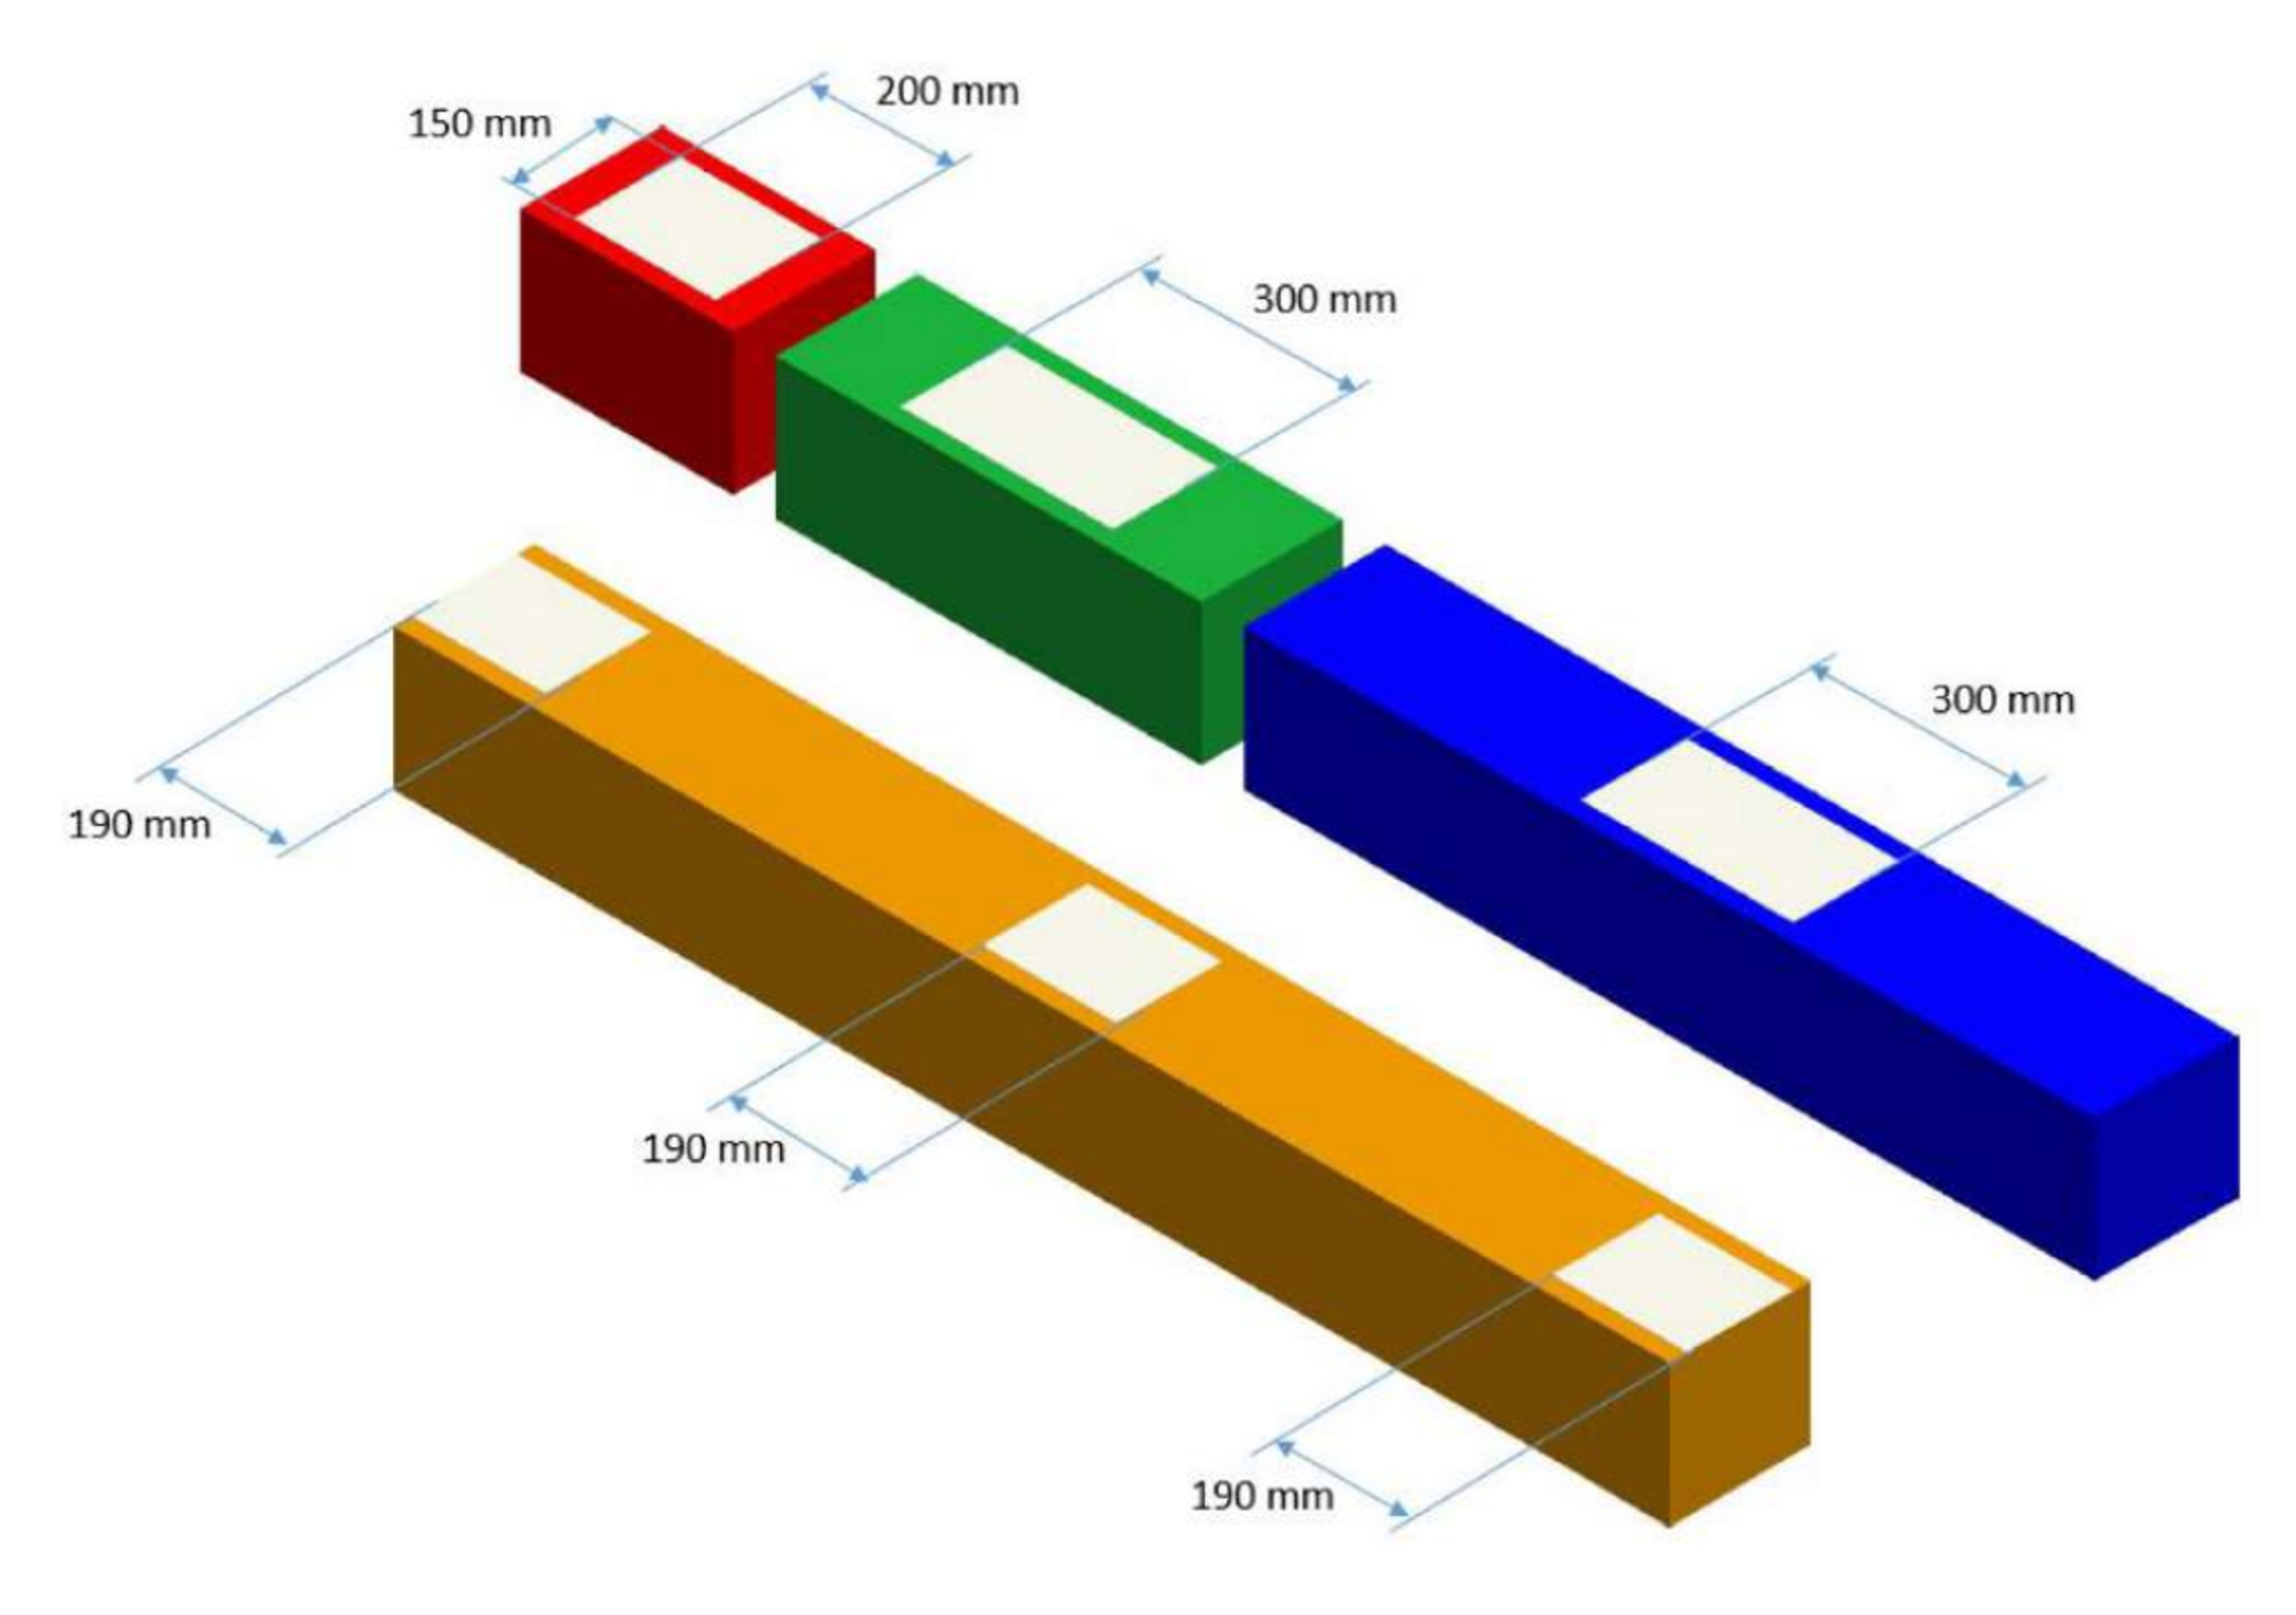
\includegraphics[scale=0.35]{fig/brick_sample.png}
\caption[Bricks definition]{Colors and dimensions of the bricks provided by the organizer.}
\label{fig:brickdef}

\end{figure}

Each brick has thin metal plate on top of it, so that the robots are able to pick them up using electromagnets. In the beginning of challenge are all bricks placed at beforehand unknown position. Initial position of bricks is unknown but there is a predefined pattern in which are the bricks put together. There are different patterns for the UGV piles of bricks and the UAV piles. The UGV bricks are stacked into the multiple height levels whereas the UAV bricks are stacked into the width and all are put on the ground. Due to the low weight of the bricks it is necessary to put UAV bricks into the rails, otherwise the bricks can be easily blown away by the propellers of the drones. Since the UAV bricks are all on the ground level (in purely horizontal pattern), it is much easier to detect them with the UAV bottom camera than using the lidar. That is why we are further concerned only about UGV bricks. These bricks are stacked in the positions displayed in the figure \ref{fig:piledef}.

\begin{figure}[H]

\centering
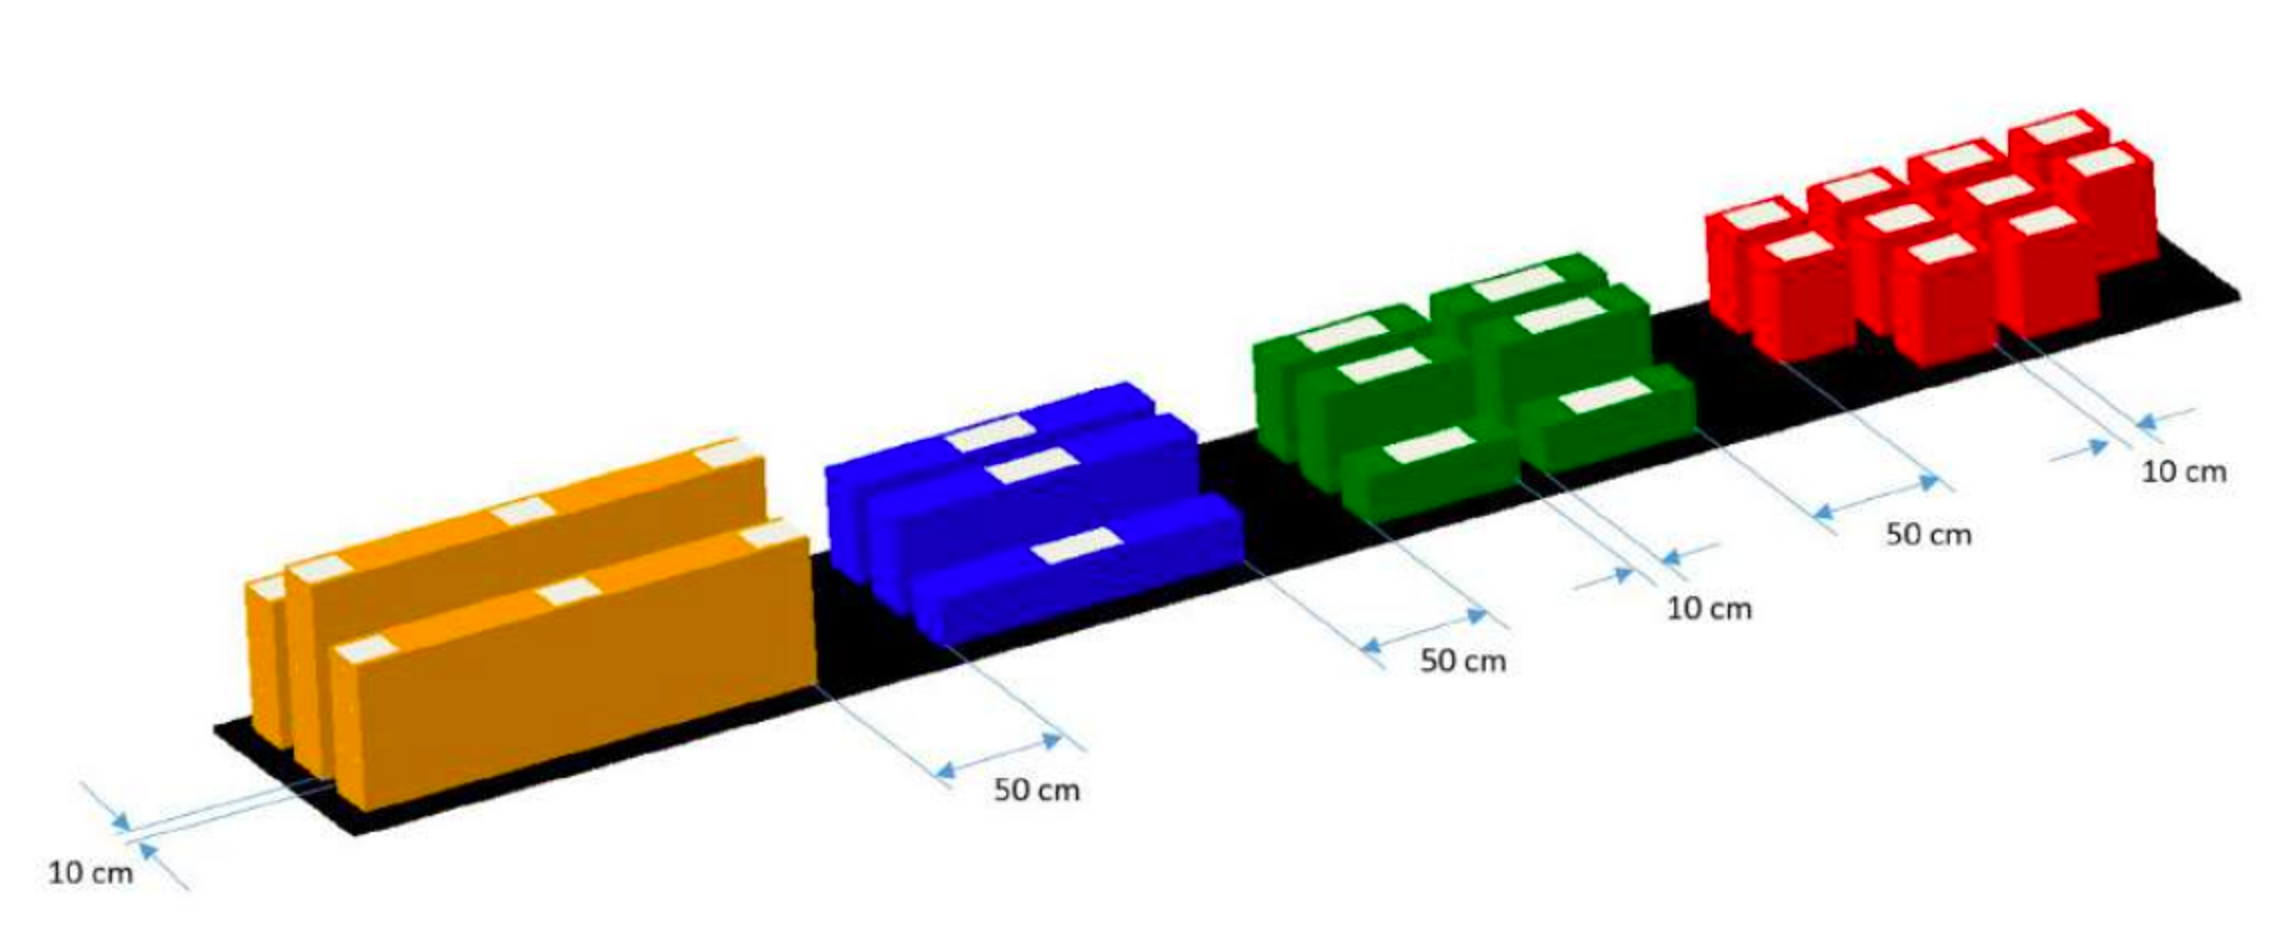
\includegraphics[scale=0.35]{fig/initial_layout.png}
\caption[Initial brick layout]{The positions of the bricks at the beginning of the second challenge.}
\label{fig:piledef}

\end{figure}

Another objects of interest are destinations where the bricks should be placed. The robots must during the exploration look for them too. UGV bricks destination is marked by checker pattern. Detecting pattern was very challenging because exact shape was not know till second rehersal. The final form of the pattern is shown in the figure \ref{fig:checker}. Although we are not concerned about the UAV bricks, the destination of the UAV bricks is a vertical object, so it is much easier to detect it from the ground using the lidar. The UAV brick destination is basically a wall as can be seen in the picture \ref{fig:uavdest}. Bricks should be placed on top of this wall. The metal plate on top of each brick shifts the center of mass to the top and make the brick very susceptible to rolling. That is why are on the top of UAV destination auxiliary handles to help place the bricks properly. At the beginning of the challenge is each team given the instructions which describe how the wall should look like at the end. When the built wall does not fit the instructions, the team gets penalty and gains less points for inaccurately placed bricks.


\begin{figure}[H]
\centering
\begin{subfigure}{.3\textwidth}
  \centering
\vspace{18mm}
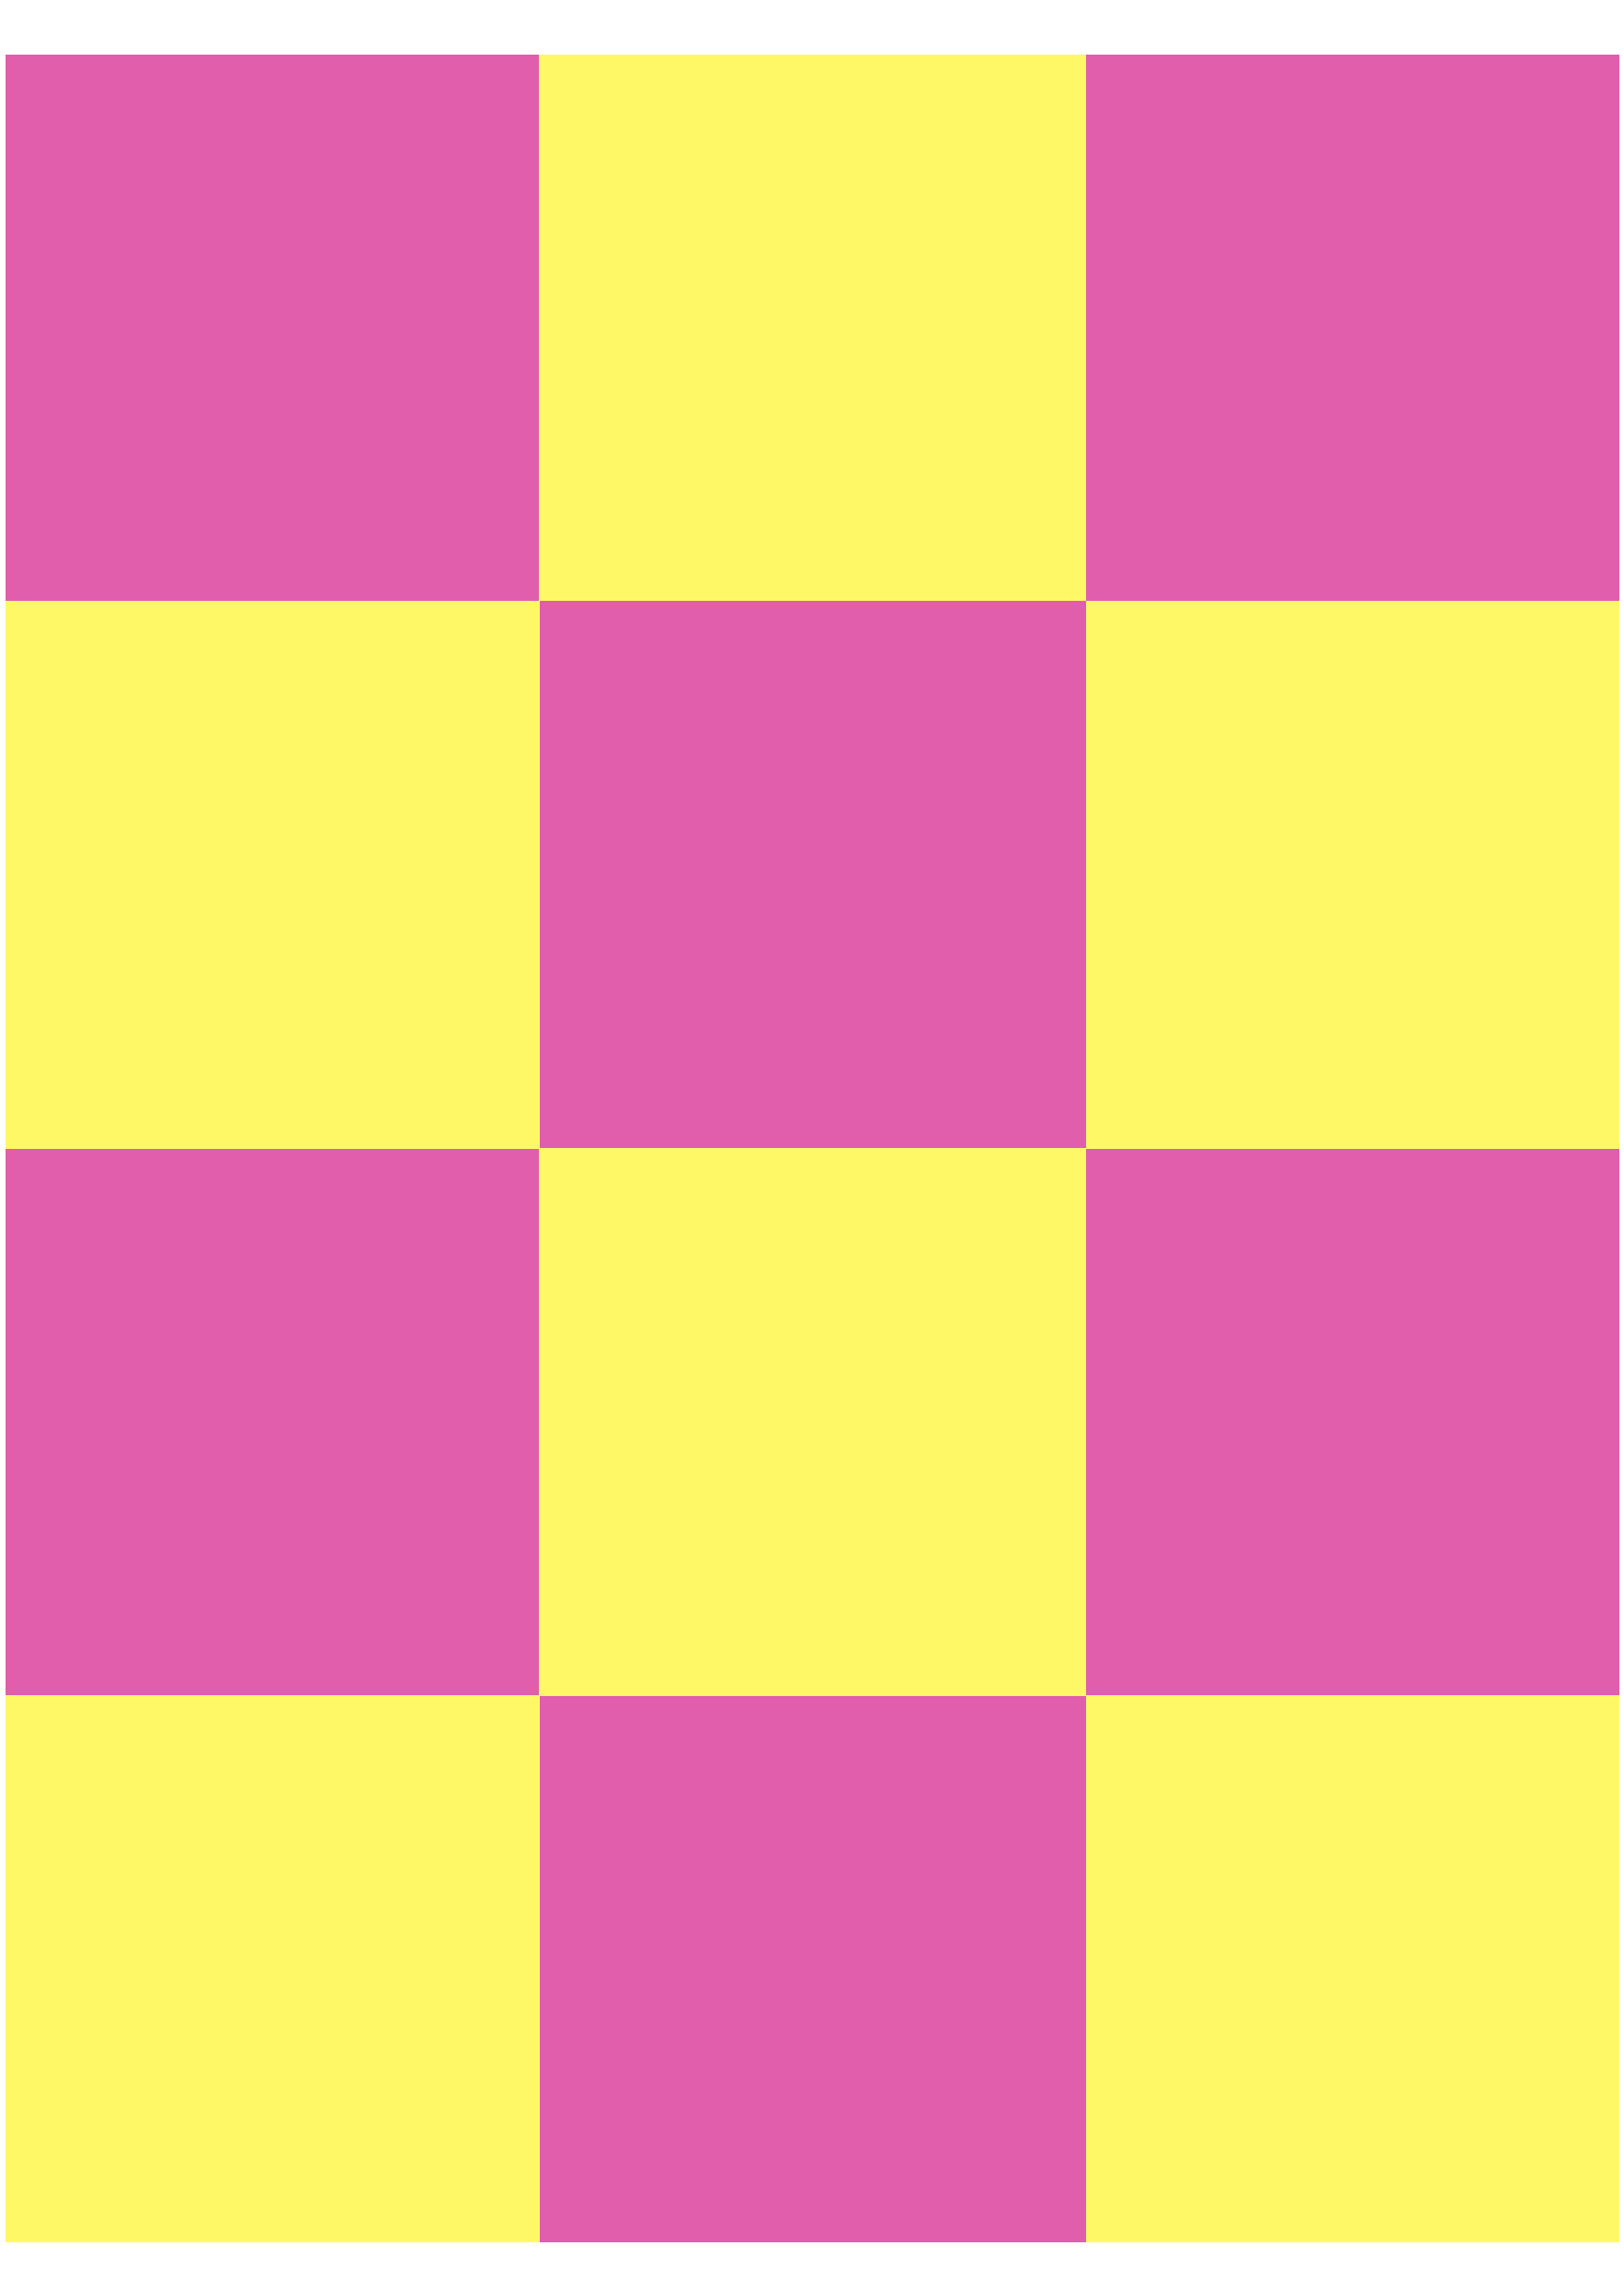
\includegraphics[scale=0.1]{fig/pattern.pdf}
\vspace{18mm}
\caption[UGV destination]{UGV destination pattern.}
\label{fig:checker}
\end{subfigure}
\begin{subfigure}{.65\textwidth}
  \centering
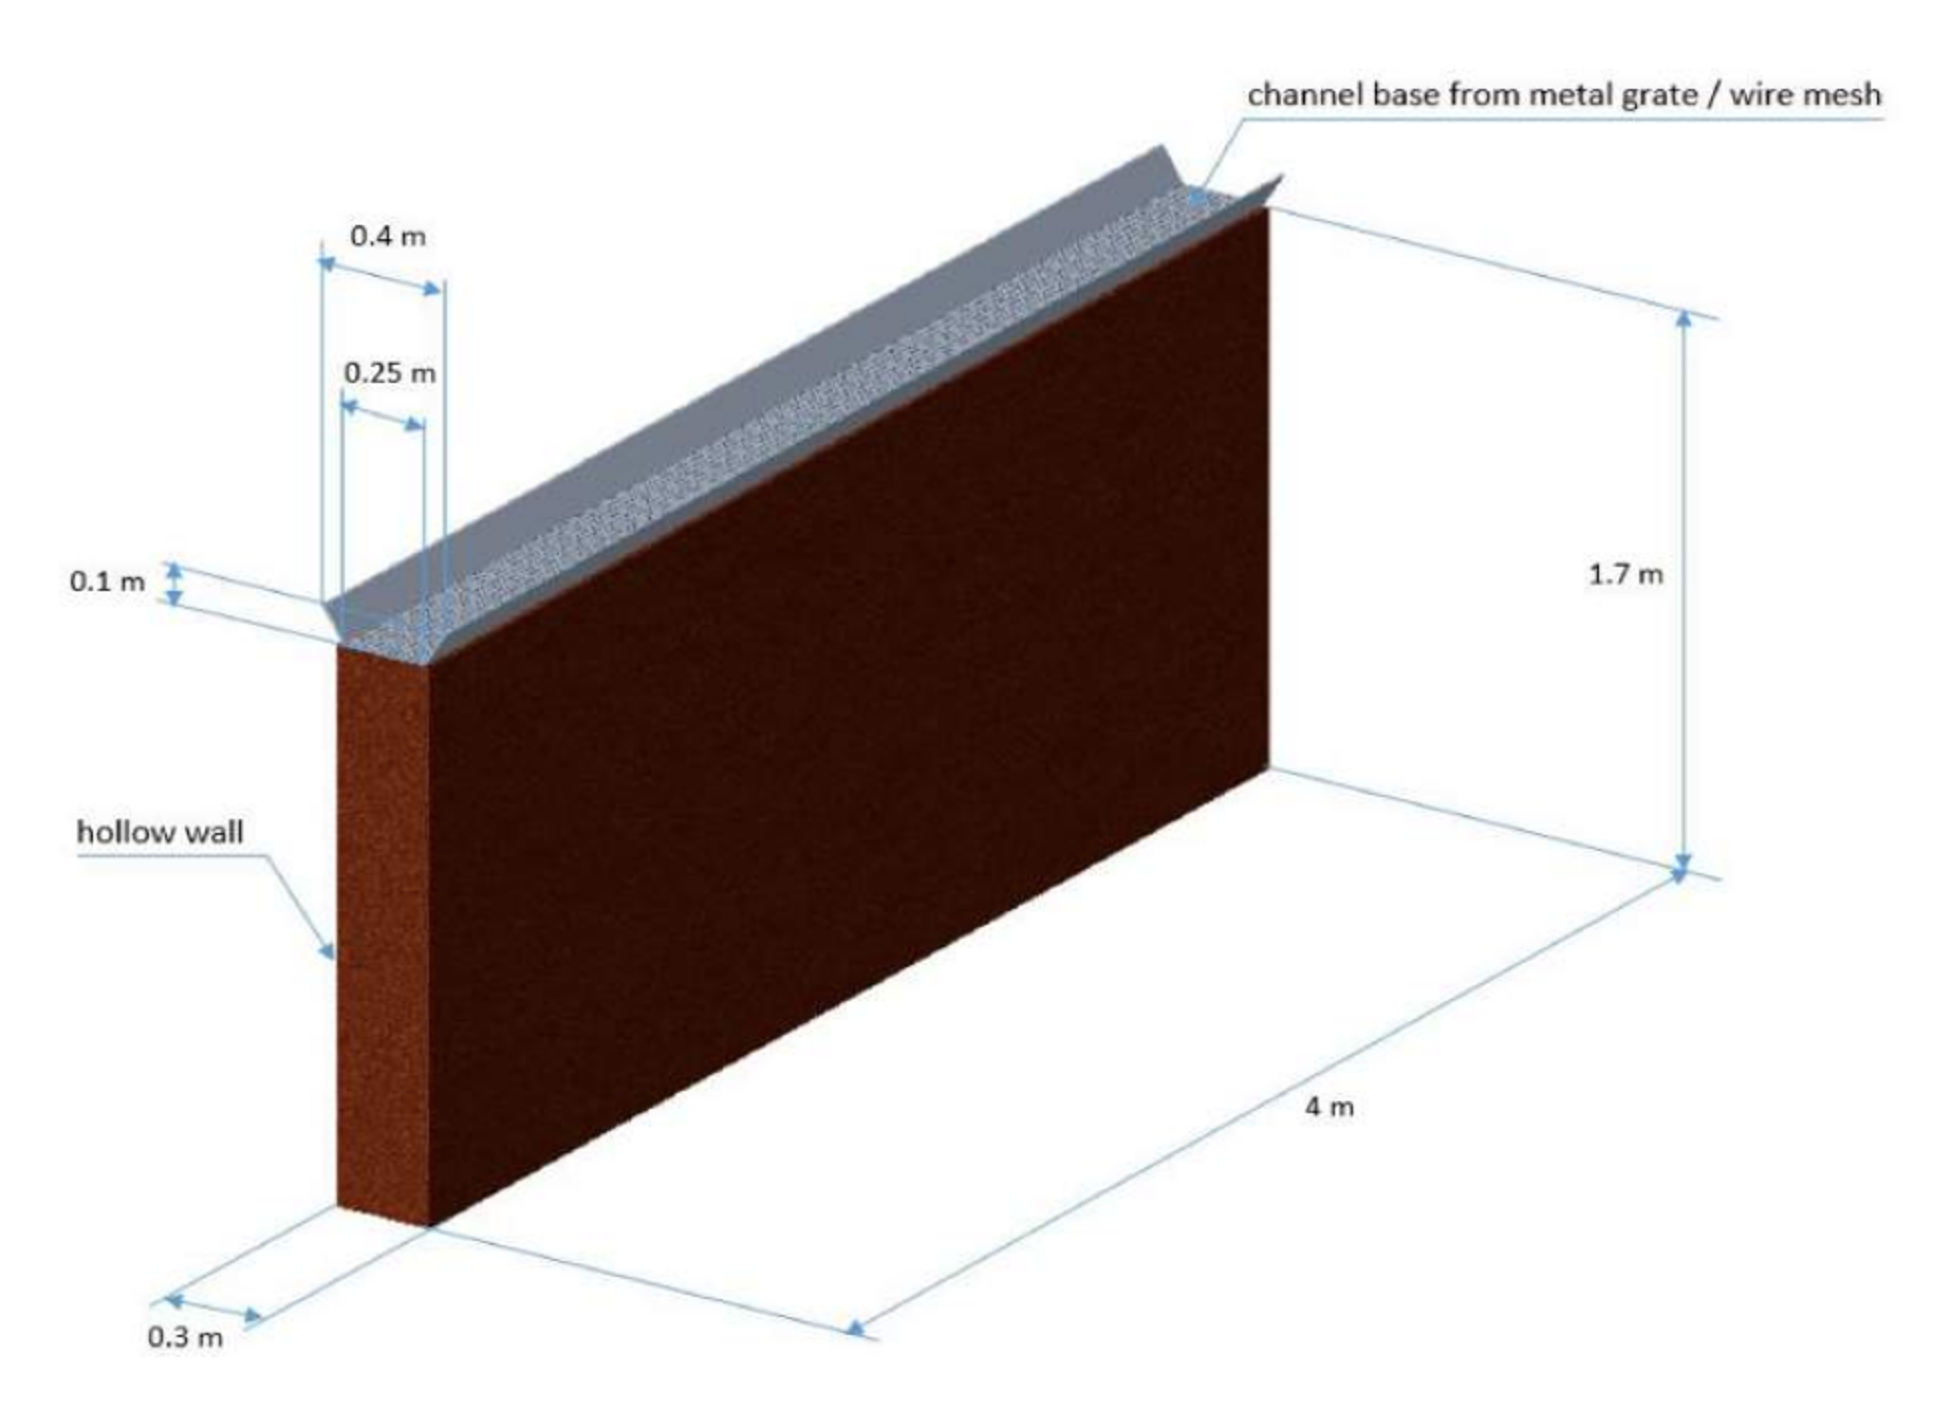
\includegraphics[scale=0.35]{fig/wall_sample.png}
\caption[UAV destination]{UAV destination}
\label{fig:uavdest}
\end{subfigure}

\caption[Brick destinations]{Description of target places for UAVs and UGVs. Each square in the UGV pattern has $10$cm. Pattern consists of two $4\times0.4$ meter segments which are connected into the \textit{L} shape. Whole UAV destination consists of five similar segments arranged into the \textit{M} shape with right angles.}
\label{fig:dest}
\end{figure}


\section{Equipment}
For the sake of completeness is necessary to describe what exact equipment was available. We used \textbf{Clearpath Husky A200} which is wheeled robot designed for outside robotics. The robot is equipped with many additional devices. As a computer running all code controlling the robot is used \textbf{Intel NUC}. To manipulate the bricks we mounted \textbf{Kinova robotic arm} on top of the Husky robot. Two \textbf{12V electromagnets} are attached to the end-effector to enable the arm to grip the bricks. It would be very hard to grip the bricks without any feedback loop to the hand. For visual servoing and proper gripping we placed \textbf{Intel Realsense} camera close to the end of the arm. It is also possible to obtain feedback from electromagnets thanks to hall effect sensors and decide whether the brick is gripped correctly. For the localization, collision avoidance and detection is used \textbf{Velodyne VLP-16} lidar sensor. Lastly for the moving the bricks around the arena we created a handmade cargo area which can contain up to six bricks and attached it to the rear bumper. It was not possible to carry more bricks mainly because of restrictions on robots size and also due to the limited range of Kinova arm. Whole setup is captured in the figure \ref{fig:husky}.

\begin{figure}[H]
\centering
\includegraphics[scale=0.3]{fig/husky.png}
\caption[UGV robot setup]{Clearpath Husky A200 adjusted for the second challenge.}
\label{fig:husky}

\end{figure}

\subsection{Velodyne VLP-16}
This thesis deals mainly with lidar data so following subsection will provide more detailed description of lidar sensor. Inside the VLP-16 puck is rotating class one infrared laser which measures the distance using the time of flight principle. Lidar is powered by 12V power supply and the data are transferred via UDP packets over the ethernet. Parameters of the Velodyne lidar are listed in the table \ref{tab:lidar}.

\begin{table}[H]
\centering
\begin{tabular}{|l|c|}
\hline
Layers                            & 16   \\ \hline
Range (m)                         & 100  \\ \hline
Vertical FOV ($\degree$)          & $\pm20$   \\ \hline
Vertical resolution ($\degree$)   & 2    \\ \hline
Horizontal FOV ($\degree$)        & 360  \\ \hline
Horizontal resolution ($\degree$) & 0.1  \\ \hline
Frequency (Hz)                    & 5    \\ \hline
Precision (m)                     & $\pm0.03$ \\ \hline
\end{tabular}
\caption{Parameters of VLP-16 lidar sensor.}
\label{tab:lidar}
\end{table}


\section{STH ABOUT ROS???}